\documentclass{article}

\usepackage{graphicx}
\usepackage{multirow}

\title{Note: Logistic Regression}
\author{Sun Zhao}

\begin{document}
\maketitle
\newpage

\section{Classification}
In classification problem, we will predict the label for the given data instead of continuous values like regression problem. For example, a classifier may automatically label an email as spam or not spam, an online transaction fraudulent or not fraudulent, or a tumor malignant or benign. In the simplest case, there are only two classes. Usually, we use 0 and 1 to denote the negative class and the positive class separately. Figure\ref{classification_example} shows a training data set of tumor classification. When using linear regression algorithm and exclude blue cross example, we get a hypothesis of purple line. Naturally, we define 0.5 as the boundary of malignant or benign, ie, if the hypothesis h(x) is equal to or greater than 0.5, then x is malignant, otherwise benign. Let $h(x_{0})$ = 0.5, then if x >= $x_{0}$, x is malignant, otherwise benign. In this case, we get a perfect classifier. However, if the blue cross is included, we may get a hypothesis of green line. And let $h(x_{1})$ = 0.5, obviously, $x_{1}$ is worth than $x_{0}$ when classifying tumors. This is because in the binary classification problem, the value of y is always 0 or 1, but the output of linear regression can be larger than 1 or smaller than 0. Logistic regression will use a hypothesis $h_{\theta}(x)$ whose output is always between 0 and 1.

\begin{figure}[ht]
  \centering
  % Requires \usepackage{graphicx}
  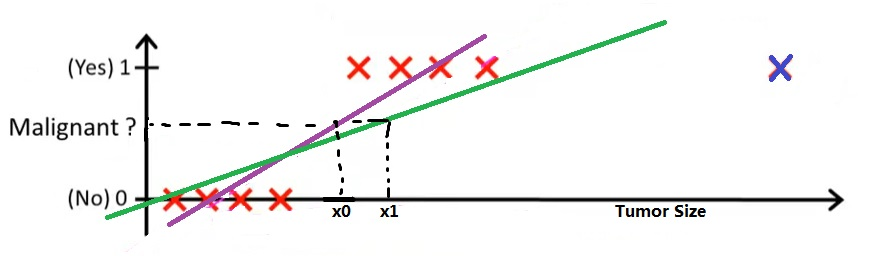
\includegraphics[width=8cm]{Figure1.jpg}\\
  \caption{}\label{classification_example}
\end{figure}

\section{Hypothesis Representation}
How to control the output of our hypothesis between 0 and 1? The answer is using a sigmoid function shown in formula\ref{sigmoid_function}. The sigmoid function plotted in Figure\ref{sigmoid_function_plotting} maps an interval of (-$\infty, \infty$) to (0, 1). Combining the sigmoid function and hypothesis function $h_{\theta}(x) = \theta^{T}x$, we will get the hypothesis function of logistic regression shown in formula\ref{logistic_regression_hypothesis}. The output of the new hypothesis $h_{\theta}(x)$  means the probability that y = 1 on input of x. For example, in the tumor classification problem, if $h_{\theta}(x_{0}) = 0.7$, then we can tell the patient whose tumor size is equal to $x_{0}$ that there are 70\% chance that her/his tumor to be malignant. Formally, the hypothesis predicts the probability of x being positive class given x and $\theta$. This definition is described in formula\ref{hypothesis_probability_definition}, and obviously, we can induce a property shown in formula\ref{probalility_property}.
\begin{equation}\label{sigmoid_function}
Sigmoid(x) = \frac{1}{1 + e^{-x}}
\end{equation}

\begin{equation}\label{logistic_regression_hypothesis}
h_{\theta}(x) = \frac{1}{1 + e^{-\theta^{T}x}}
\end{equation}

\begin{equation}\label{hypothesis_probability_definition}
h_{\theta}(x) = P(y = 1|x;\theta)
\end{equation}

\begin{equation}\label{probalility_property}
P(y = 0|x;\theta) + P(y = 1|x;\theta) = 1
\end{equation}
\begin{figure}[ht]
  \centering
  % Requires \usepackage{graphicx}
  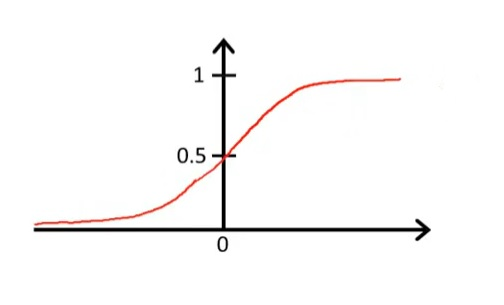
\includegraphics[width=8cm]{Figure2.jpg}\\
  \caption{}\label{sigmoid_function_plotting}
\end{figure}
\end{document}
